\documentclass[tikz,border=4pt]{standalone}
\usepackage{libertine}
\usetikzlibrary{arrows.meta,calc,positioning,fit,backgrounds,shapes.geometric}
\definecolor{paperink}{HTML}{263441}
\definecolor{papermuted}{HTML}{647481}
\definecolor{paperline}{HTML}{CCD5DB}
\definecolor{paperblue}{HTML}{2D5F91}
\definecolor{paperbluefill}{HTML}{EFF5FA}
\definecolor{paperorange}{HTML}{B66731}
\definecolor{paperorangefill}{HTML}{FCF4EB}
\definecolor{papergreen}{HTML}{3F7558}
\definecolor{papergreenfill}{HTML}{EFF6F1}
\tikzset{
  papertext/.style={font=\footnotesize, text=paperink},
  papermini/.style={font=\scriptsize, text=papermuted},
  paneltitle/.style={font=\footnotesize\bfseries, text=paperink},
  bluebox/.style={draw=paperblue, fill=paperbluefill, rounded corners=1pt,
    line width=.6pt, font=\footnotesize, text=paperink, align=center,
    inner xsep=6pt, inner ysep=5pt},
  orangebox/.style={draw=paperorange, fill=paperorangefill, rounded corners=1pt,
    line width=.6pt, font=\footnotesize, text=paperink, align=center,
    inner xsep=6pt, inner ysep=5pt},
  greenbox/.style={draw=papergreen, fill=papergreenfill, rounded corners=1pt,
    line width=.6pt, font=\footnotesize, text=paperink, align=center,
    inner xsep=6pt, inner ysep=5pt},
  graybox/.style={draw=paperline, fill=white, rounded corners=1pt,
    line width=.6pt, font=\footnotesize, text=paperink, align=center,
    inner xsep=6pt, inner ysep=5pt},
  orangeflow/.style={-{Stealth[length=2mm]}, draw=paperorange, line width=1pt},
  blueflow/.style={-{Stealth[length=2mm]}, draw=paperblue, line width=1.15pt},
  greenflow/.style={-{Stealth[length=2mm]}, draw=papergreen, line width=1pt},
  grayflow/.style={-{Stealth[length=1.8mm]}, draw=papermuted, line width=.65pt}
}

\begin{document}
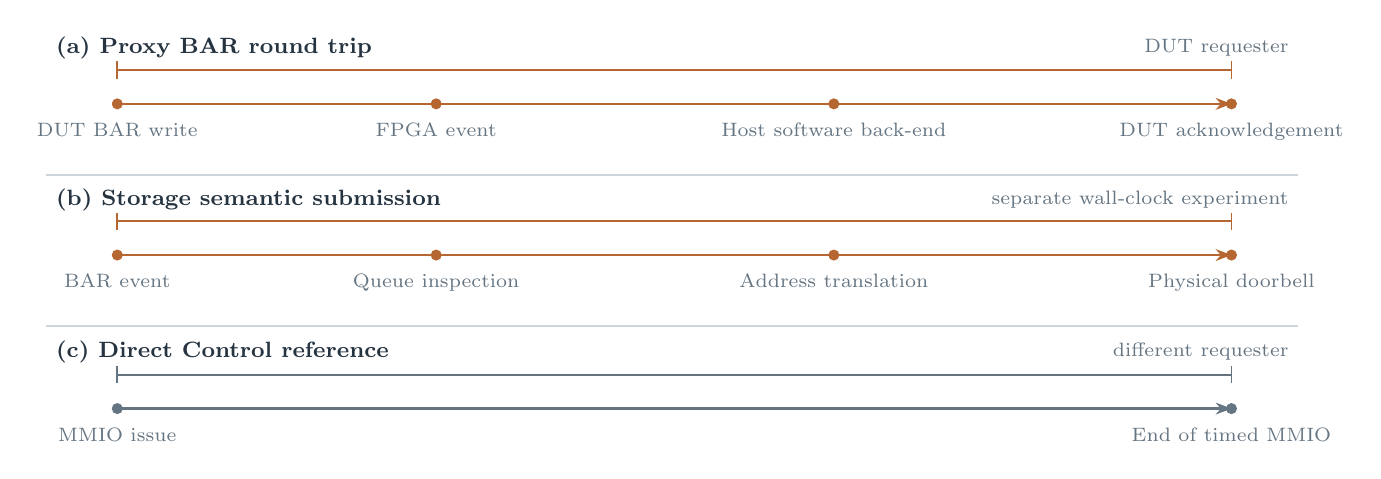
\begin{tikzpicture}[x=1cm,y=1cm]
  \node[paneltitle, anchor=west] at (.1,5.06) {(a) Proxy BAR round trip};
  \node[papermini, anchor=east] at (16.0,5.06) {DUT requester};
  \draw[paperorange, line width=.95pt, -{Stealth[length=2mm]}]
    (1.0,4.35) -- (15.15,4.35);
  \foreach \x/\lab in {1.0/{DUT BAR write},5.05/{FPGA event},10.10/{Host software back-end},15.15/{DUT acknowledgement}} {
    \fill[paperorange] (\x,4.35) circle (2pt);
    \node[papermini, anchor=north] at (\x,4.23) {\lab};
  }
  \draw[paperorange, line width=.65pt] (1.0,4.78) -- (15.15,4.78);
  \draw[paperorange, line width=.65pt] (1.0,4.67) -- (1.0,4.89);
  \draw[paperorange, line width=.65pt] (15.15,4.67) -- (15.15,4.89);

  \draw[paperline, line width=.65pt] (.1,3.45) -- (16.0,3.45);
  \node[paneltitle, anchor=west] at (.1,3.13) {(b) Storage semantic submission};
  \node[papermini, anchor=east] at (16.0,3.13) {separate wall-clock experiment};
  \draw[paperorange, line width=.95pt, -{Stealth[length=2mm]}]
    (1.0,2.43) -- (15.15,2.43);
  \foreach \x/\lab in {1.0/{BAR event},5.05/{Queue inspection},10.10/{Address translation},15.15/{Physical doorbell}} {
    \fill[paperorange] (\x,2.43) circle (2pt);
    \node[papermini, anchor=north] at (\x,2.31) {\lab};
  }
  \draw[paperorange, line width=.65pt] (1.0,2.86) -- (15.15,2.86);
  \draw[paperorange, line width=.65pt] (1.0,2.75) -- (1.0,2.97);
  \draw[paperorange, line width=.65pt] (15.15,2.75) -- (15.15,2.97);

  \draw[paperline, line width=.65pt] (.1,1.53) -- (16.0,1.53);
  \node[paneltitle, anchor=west] at (.1,1.20) {(c) Direct Control reference};
  \node[papermini, anchor=east] at (16.0,1.20) {different requester};
  \draw[papermuted, line width=.8pt, -{Stealth[length=2mm]}]
    (1.0,.48) -- (15.15,.48);
  \fill[papermuted] (1.0,.48) circle (2pt);
  \fill[papermuted] (15.15,.48) circle (2pt);
  \node[papermini, anchor=north] at (1.0,.36) {MMIO issue};
  \node[papermini, anchor=north] at (15.15,.36) {End of timed MMIO};
  \draw[papermuted, line width=.65pt] (1.0,.91) -- (15.15,.91);
  \draw[papermuted, line width=.65pt] (1.0,.80) -- (1.0,1.02);
  \draw[papermuted, line width=.65pt] (15.15,.80) -- (15.15,1.02);
\end{tikzpicture}
\end{document}
